\documentclass{article}
\usepackage{ja}
%\usepackage{epsfig} %(this is to import figures)
%\usepackage{graphicx}
\usepackage[dvips]{graphicx}
% Latex en español
%\usepackage[spanish,activeacute]{babel}
%\usepackage[ansinew]{inputenc}
\usepackage[utf8]{inputenc} % Lo puse para que se reconozcan directamente los acentos

\title{INSTRUCCIONES PARA LOS AUTORES (14ptos, negrita)}

\author{Autor (10ptos)\\Direcci\'{o}n, e-mail (10ptos) \\ \\ Coautor(10ptos)\\ Direcci\'{o}n, e-mail(10ptos)}

\begin{document}

\maketitle

\begin{abstract}
{\em El párrafo correspondiente al resumen debe tener un tipo de
letra de 10 puntos, en it\'{a}lica. La palabra {\bf Resumen} debe
estar centrada, y separada tres l\'{\i}neas de la \'{u}ltima
direcci\'{o}n de autor. Entre el t\'{\i}tulo y el primer autor dejar
un espacio de dos l\'{\i}neas.}

{\bf Palabras clave:} Dejar tres l\'{\i}neas entre esta frase y la primera
separaci\'{o}n.\\
\end{abstract}

\section{INSTRUCCIONES GENERALES DEL FORMATO (12 ptos, negrita)}
Los trabajos deben estar en formato de papel de 21 cm x 29.7 cm.
El texto debe estar escrito en Times New Roman a 10 puntos, y a dos
columnas, con un ancho total de 16 cm; cada columna debe tener
un ancho de 7.6 cm, con un espacio entre columnas de 0.8 cm. El texto
tendr\'{a} un interlineado sencillo y deber\'{a} estar justificado. Dejar
una l\'{\i}nea entre p\'{a}rrafos.

El margen superior debe ser de 2.5 cm y el inferior de 3 cm. Los m\'{a}rgenes
izquierdo y derecho deben ser de 2.5 cm.

\section{SECCIONES, NOTAS, CITAS, FIGURAS, F\'{O}RMULAS, TABLAS Y REFERENCIAS (12ptos, negrita)}

\subsection{SECCIONES Y SUBSECCIONES}

\subsubsection{Subsecci\'{o}n}

Si hubiera m\'{a}s subsecciones, tendr\'{\i}an el mismo formato que \'{e}sta subsecci\'{o}n.
Tanto los t\'{\i}tulos de las secciones como los de la subsecciones est\'{a}n con
sangr\'{\i}a y alineados a la izquierda.

\subsection{NOTAS A PIE DE P\'{A}GINA}

No incluir cabecera ni pie de p\'{a}gina.

\subsection{CITAS EN EL TEXTO}

Las citas dentro del texto deben incluir el n\'{u}mero de referencia entre
corchetes, por ejemplo \cite{bibli1}.

\subsection{FIGURAS}

Todas las figuras deben estar centradas y ser claras. El n\'{u}mero de la
figura y la leyenda aparecer\'{a}n siempre en la parte inferior de la
figura. Cada figura debe ser numerada correlativamente y debe estar
referenciada en el texto. Dejar una l\'{\i}nea entre el texto del p\'{a}rrafo
y la figura.

\begin{figure}[htbp]
%\centerline{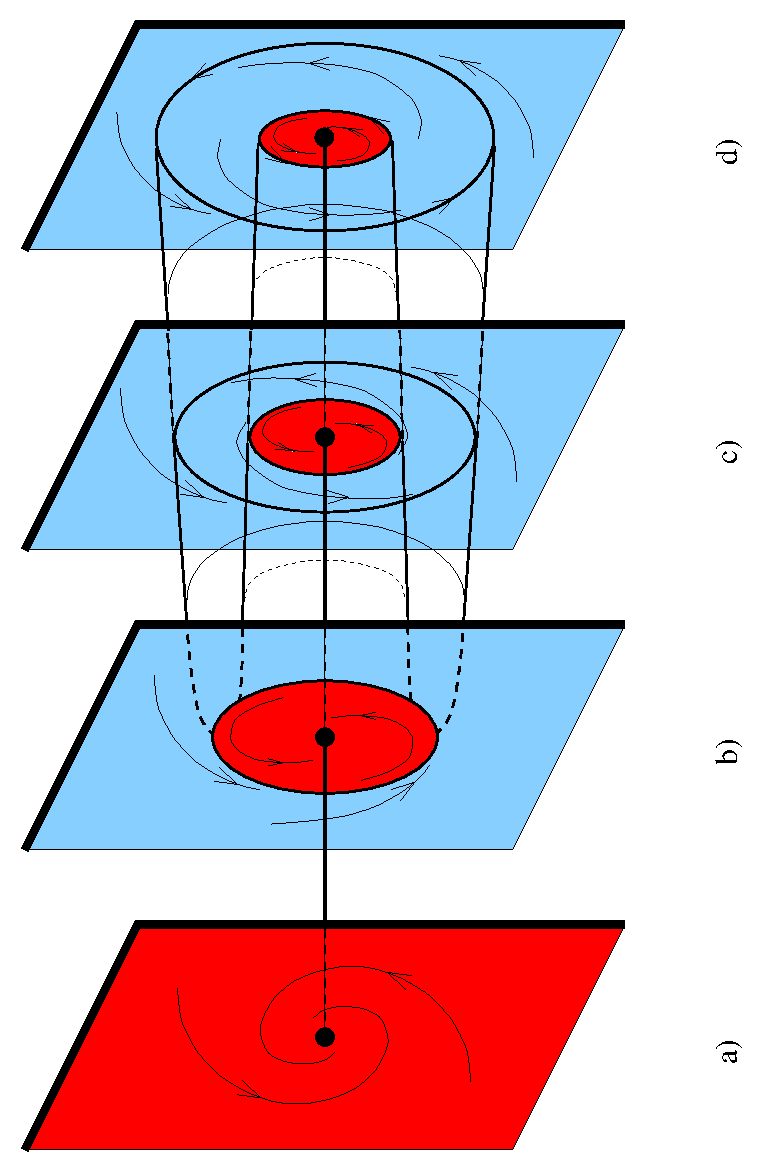
\psfig{file=figure1.eps,width=3cm,height=3cm,angle=-90}}
\centerline{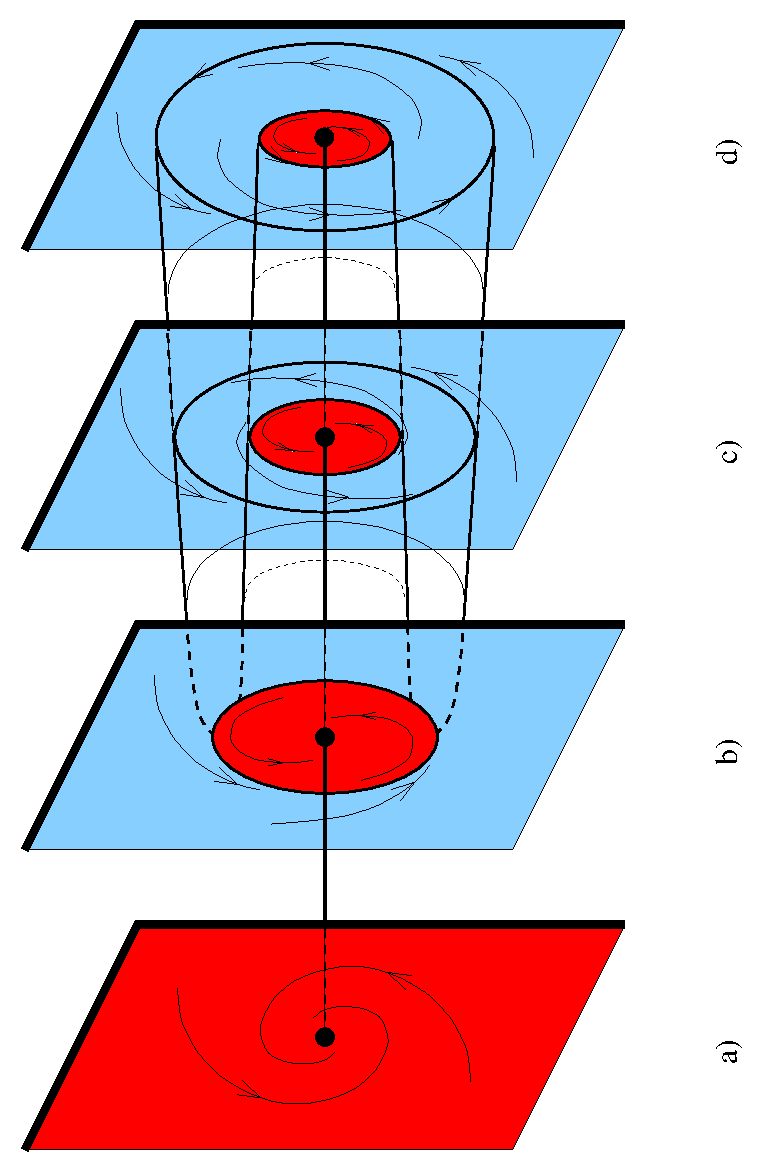
\includegraphics[width=3cm,height=3cm,angle=-90]{figure1}}
\caption{Ejemplo de leyenda de una figura} \label{fig:1}
\end{figure}



\subsection{F\'{O}RMULAS}

Las f\'{o}rmulas deben estar centradas y numeradas correlativamente, dejando
una l\'{\i}nea entre el texto y la f\'{o}rmula tanto antes como despu\'{e}s, o entre
dos f\'{o}rmulas consecutivas. Referenciar las ecuaciones mediante su numeraci\'{o}n.
\begin{eqnarray}
\mu_A(x) & = & \exp \left( \frac{-(x-\mu_A(x))^2}{2\sigma_A^2} \right)
\end{eqnarray}

\subsection{TABLAS}

Todas las tablas tienen que estar referenciadas en el texto, como se
ha hecho en la tabla ~\ref{ttabl}, centradas y claras. El n\'{u}mero y t\'{\i}tulo
siempre aparecer\'{a}n en la parte superior de la tabla, dejando un espaciado
de una l\'{\i}nea entre el texto del p\'{a}rrafo y la tabla. Las tablas deben estar
numeradas de manera correlativa.

\begin{table}[ht]
\begin{center}
\caption{Ejemplo de t\'{\i}tulo de una tabla.}\label{ttabl}
\begin{tabular}{|c|l|}
   \hline
   {\bf Nombre} & {\bf Descripci\'{o}n} \\ \hline $A$ &   Subconjunto borroso de $X$\\
   $\mu_{A}$ & Funci\'{o}n de pertenencia de$A$ \\
   \hline
\end{tabular}
\end{center}
\end{table}

\begin{acknowl}
La palabra {\bf Agradecimientos} debe ir alineada a la izquierda,
no numerada y en negrita. todos los agradecimientos deben figurar al final
del trabajo.
\end{acknowl}

\begin{eng}

\large\bf{TITLE OF THE PAPER IN ENGLISH (12 ptos, negrita)}\bigskip

\large\bf{Abstract}\bigskip
\normalfont

{\em Summary of the paper in English.} \bigskip

{\bf Keywords:} Leave three lines between this sentence and the following section.

\end{eng}\bigskip

\begin{thebibliography}{99}

\bibitem{bibli1} Pedrycz, W., (1993) Fuzzy sets and fuzzy systems,
Research Studies Press, England.

\bibitem{bibli2} Zadeh, L., (1965) ``Fuzzy logic'',
{\em Fuzzy Sets and Systems}, pp 100-106.

\end{thebibliography}

Deben estar ordenadas por orden alfab\'{e}tico y justificadas con la sangr\'{\i}a correspondiente.


%Copyright (no borrar)

\vspace{1cm}
\setbox0\vbox{\noindent

\includegraphics[width=0.18\textwidth]{logo-cc-by-nc-sa}}
\wd0=0pt\ht0=0pt\box0
\hangindent=33mm\hangafter =-3\vspace{-4mm} 
\small
\copyright{}{\@ \the\year} by the authors. Submitted for possible open access publication under the terms and conditions of the Creative Commons Attribution CC BY-NC-SA 4.0 license (https://creativecommons.org/licenses/by-nc-sa/4.0/deed.es).

\end{document}
